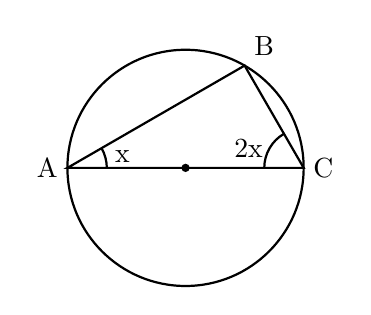
\begin{tikzpicture}[scale=1]

  % Define the center of the circle
  \coordinate (O) at (0,0);

  % Define the radius of the circle
  \def\R{1.5}

  % Draw the circle
  \draw[thick] (O) circle (\R);

  % Add a dot at the center
  \fill (O) circle (1.5pt);

  % Define the vertices of the inscribed triangle
  % A and C are on the horizontal diameter
  \coordinate (A) at (-\R, 0);
  \coordinate (C) at (\R, 0);
  
  % B is on the circle. Based on the angles (x and 2x), angle at C is 2x and angle at A is x.
  % Since AC is a diameter, the angle at B is 90 degrees.
  % So x + 2x + 90 = 180 => 3x = 90 => x = 30 degrees.
  % Angle at A is 30, Angle at C is 60.
  % The coordinates of B can be found using the angle.
  % From center O, the angle to B is 180 - 2*30 = 120 or 2*60 = 120.
  % Let's place B at angle 60 from center to match the visual representation
  \coordinate (B) at (60:\R);

  % Draw the triangle ABC
  \draw[thick] (A) -- (B) -- (C) -- cycle;

  % Draw the diameter AC (already drawn as part of the triangle, but ensures it passes through center)
  \draw[thick] (A) -- (C);

  % Draw the arc for angle x at A
  % The angle at A is approximately 30 degrees
  \draw[thick] (-1.0, 0) arc (0:30:0.5);
  \node at (-0.8, 0.15) {x};

  % Draw the arc for angle 2x at C
  % The angle at C is approximately 60 degrees, from 180 to 120
  \draw[thick] (1.0, 0) arc (180:120:0.5);
  \node at (0.8, 0.25) {2x};

  % Add labels for the vertices
  \node[left] at (A) {A};
  \node[above right] at (B) {B};
  \node[right] at (C) {C};

\end{tikzpicture}